\section{General numerical methods}
\subsection{Polynomial approximation}
A polynomial approximation is an approximation of a curve or a function with a polynomial. In this section we will see how to find a family of polynomials widely used to estimate functions, known as Taylor polynomials or Taylor series.



\subsubsection{Linear and quadratic approximation}
Let's start with approximating a function using its tangent line - a key idea in Euler's method. Assume that we know the function value and its derivative at some point (e.g. $f(a), f'(a)$). We can use these to approximate $f(x)$ for other points $x$ relatively near $a$ by:
\begin{equation}
	f(x) \approx P_1(x) = f(a) + f'(a)(x-a)
\end{equation}
This is called the first order Taylor polynomial of $f(x)$.

To get a better approximation, we can try to use a quadratic polynomial. Another thing we can try is to find a polynomial that has the same value as the function at some point $a$ and the same first and second derivatives there. We can do both by defining the second order Taylor polynomial for $f(x)$ near the point $x = a$ as follows:
\begin{equation}
	f(x) \approx P_2(x) = f(a) + f'(a)(x-a) + \frac{f''(a)}{2}(x-a)^2
\end{equation}



\subsubsection{Higher-order approximation}
By involving more derivatives and getting higher order polynomial we get better and better polynomial approximation. The $n$-th order Taylor polynomial for $x$ near $a$ is given by:
\begin{equation}
	P_n(x) = f(a) + f'(a)(x-a) + \frac{f''(a)}{2}(x-a)^2 + \sum_{i=3}^n \frac{f^{(i}(a)}{i!}(x-a)^i
\end{equation}
As $n$ goes to infinity, we have the \href{https://en.wikipedia.org/wiki/Taylor_series}{Taylor series}. The Taylor series is defined as follows:

\begin{center}
\begin{footnotesize}
\fbox{
\begin{minipage}{0.90\textwidth}

The Taylor series of a real or complex-valued function $f(x)$ that is infinitely differentiable at a real or complex number $a$ is the power series:
\begin{equation}
	P_n(x) = \sum_{n=0}^\infty \frac{f^{(n)}(a)}{n!}(x-a)^n
\end{equation}
where $f^{(n)}(a)$ denotes the $n$-th derivatives of $f$ evaluated at the point $a$. The derivative of order zero of $f$ is defined to be $f$ itself. 

\end{minipage}
}
\end{footnotesize}
\end{center}

Examples of Taylor series for several functions at $a = 0$ are given below:
\begin{itemize}
	\item Single function:
	\begin{itemize}
		\item $e^{x} = \sum_{n=0}^\infty \frac{x^n}{n!} = 1 + x + \frac{x^2}{2} + \frac{x^3}{6} + R_4(x)$
		\item $\ln(1+x) = \sum_{n=0}^\infty (-1)^{n+1} \frac{x^n}{n} = x - \frac{x^2}{2} + \frac{x^3}{3} + R_4(x)$
		\item $\cos(x) = \sum_{n=0}^\infty \frac{(-1)^n}{(2n)!} x^{2n}$
	\end{itemize} 
	\item A function of a function (derivation can be found in Section 14 of \href{https://en.wikipedia.org/wiki/Taylor_series}{this link}:
	\begin{itemize}
		\item $\frac{e^x}{\cos(x)} = 1 + x + x^2 + \frac{2x^3}{3} + \frac{x^4}{2} + R_5(x)$
		\item $\ln(1 + (\cos(x) - 1)) = -\frac{x^2}{2} - \frac{x^4}{12} - \frac{x^6}{45} + R_8(x)$
\end{itemize} 
\end{itemize}
The notation $R_n(x)$ is presented in the next section.



\subsubsection{Residual}
To evaluate how good the approximation is (or how big the error is) we need to calculate the difference between the approximation value and the exact answer. When using the $n$-th order Taylor series $P_n(x)$ centered at $a$ to approximate $f(x)$, the error is:
\begin{equation}
	E = f(x) - P_n(x)
\end{equation}
Often we are only interested in the magnitude of the error $|E|$. Fortunately, there is a simple formula for a bound on the size of the error $|E| = \left| R_n(x) \right|$, the bound is called the residual and is given as:
\begin{equation}
	\left| R_n(x) \right| = \left| \frac{f^{(n+1)}(c)}{(n+1)!}(x-a)^{n+1} \right|
\end{equation}
where $c$ is between $x$ and $a$. Normally, we will chose the value of $c$ in the range $(a;x)$ to maximize the value of $f^{(n+1)}(c)$; or, just choose a value that we know is surely reasonably larger than $f^{(n+1)}(c)$ for all $c \in (a;x)$. 

\begin{center}
\begin{footnotesize}
\fbox{
\begin{minipage}{0.90\textwidth}

\href{http://www.math.smith.edu/~rhaas/m114-00/chp4taylor.pdf}{\textbf{Example}}

Let's consider the magnitude of $R_5(x)$ of function $f = \cos(x)$ at $a = \pi$. We have $f^{(6)(x)} = -\sin(x)$ and $-1 \leq \sin(x) \leq 1$ hence:
\begin{equation}
	\left| f(x) - P_5(x) \right| \leq \left| R_n(x) \right| = \left| \frac{f^{(6)}(c)}{6!}(x-\pi)^6 \right| = \frac{1}{6!}(x-\pi)^6
	\nonumber
\end{equation}

If we approximate $\cos(3)$ by the fifth order Taylor series centered at $\pi$ then we have an error of at most:
\begin{equation}
	\frac{1}{720}(\pi - 3)^6 \approx 1.11 \times 10^{-9}
	\nonumber
\end{equation}

But if we approximate $\cos(1)$ also by the fifth order Taylor series centered at $\pi$ then we have an error of at most:
\begin{equation}
	\frac{1}{720}(\pi - 1)^6 \approx 3.0 \times 10^{-4}
	\nonumber
\end{equation}

\end{minipage}
}
\end{footnotesize}
\end{center}



\subsubsection{Multivariate Taylor series}
The Taylor series may also be generalized to functions of more than one variable as done in Section 19 of \href{https://en.wikipedia.org/wiki/Taylor_series}{this link}. Since the generalized equation is quite lengthy, an example for a two-variable function is given here.

Let's a function $f(x,y)$ depend on two variables $x$ and $y$, then the second order Taylor series at point $(a,b)$ is:
\begin{align}
	f(a,b) &+ (x-a)f_x(a,b) + (y-b)f_y(a,b) \nonumber \\
	       &+ \frac{1}{2!} \left( (x-a)^2 f_{xx}(a,b) + 2(x-a)(y-b) f_{xy}(a,b) + (y-b)^2 f_{yy}(a,b) \right)
\end{align}
where the subscripts denote the respective partial derivatives. A second order Taylor series expansion of a scalar-valued function of more than one variable can be written compactly as:
\begin{equation}
	T(\mathbf{x}) = f(\mathbf{a}) + (\mathbf{x-a})^T D f(\mathbf{a}) + \frac{1}{2!} (\mathbf{x-a})^T \left\{ D^2 f(\mathbf{a}) \right\} (\mathbf{x-a}) 
\end{equation}
where $D f(\mathbf{a})$ is the \href{https://en.wikipedia.org/wiki/Gradient}{gradient} of $f$ evaluated at $\mathbf{x = a}$ and $D^2 f(\mathbf{a})$ is the \href{https://en.wikipedia.org/wiki/Hessian_matrix}{Hessian matrix}. And from these two equations, you can deduce how the higher order Taylor series expansions look like for multivariate functions. 

\begin{center}
\begin{footnotesize}
\fbox{
\begin{minipage}{0.90\textwidth}

\href{http://www.math.smith.edu/~rhaas/m114-00/chp4taylor.pdf}{\textbf{Example}}

Let's practice the Taylor series expansion for a two-variable function $f(x,y) = e^x \ln(1+y)$ centered at $(a,b) = (0,0)$.

First we need to calculate the partial derivatives of $f(x,y)$ and evaluate them at the origin $(a,b)$.
\begin{alignat*}{4}
	& f_x    &&= e^{x} \ln(1+y)             && \quad \rightarrow f_x(0,0)    &&= 0  \\
	& f_y    &&= \frac{e^{x}}{1+y}          && \quad \rightarrow f_y(0,0)    &&= 1  \\
	& f_{xx} &&= e^{x} \ln(1+y)             && \quad \rightarrow f_{xx}(0,0) &&= 0  \\
	& f_{yy} &&= -\frac{e^{x}}{(1+y)^2}     && \quad \rightarrow f_{yy}(0,0) &&= -1 \\	
	& f_{xy} &&= f_{yx} = \frac{e^{x}}{1+y} && \quad \rightarrow f_{xy}(0,0) &&= f_{xy}(0,0) = 1	
\end{alignat*}

Substituting these values in to the general formula to get:
\begin{equation}
	e^{x} \ln(1+y) = T(x,y) = y + xy - \frac{y^2}{2} + ...
	\nonumber
\end{equation}

Now if we assume $(x,y) = (0.2, 0.2)$ and use this formula to approximate $e^{x} \ln(1+y)$ we will have a value of 0.220, the error is $2.69 \times 10^{-3}$.

\end{minipage}
}
\end{footnotesize}
\end{center}



\subsection{Polynomial interpolation}
This section describes the \href{https://en.wikipedia.org/wiki/Lagrange_polynomial}{Lagrange polynomials} which are widely used for polynomial interpolation. For a given set of points $(x_{j},y_{j})$, the Lagrange polynomial is the polynomial of lowest degree that assumes at each value $x_{j}$ there is a corresponding value $y_{j}$, so that the functions coincide at each point.

Given a set of $k+1$ data points:
\begin{equation}
	(x_0,y_0), (x_1,y_1),... ..., (x_k,y_k)
\end{equation}
where no two $x_i$ are the same, the interpolation polynomial in the Lagrange form is a linear combination:
\begin{equation}
	L(x) = \sum_{j=0}^k y_j l_j(x)
\end{equation}
of Lagrange basis polynomials:
\begin{equation}
	l_j(x) = \prod_{o \leq m \leq k} \frac{x - x_m}{x_j - x_m}
\end{equation}
where $0 \leq j \leq k$ and $m \neq j$.

It can be seen that, for all $j \neq i$, we have $l_j(x_i) = 0$ whereas $l_j(x_j) = 1$. It follows that $y_j l_j(x_j) = y_j$ so at each point $x_j$ we have $L(x_j) = y_j$ showing that $L$ interpolates the function exactly.

\begin{center}
\begin{footnotesize}
\fbox{
\begin{minipage}{0.90\textwidth}

\href{https://en.wikipedia.org/wiki/Lagrange_polynomial}{\textbf{Example}}

We wish to interpolate function $y = f(x)$ over the range $1 \leq x \leq 3$ given these three points:
\begin{alignat*}{4}
	& x_0 &&= 1 && \quad \rightarrow f(x_0) &&= 1  \\
	& x_1 &&= 2 && \quad \rightarrow f(x_1) &&= 4  \\
	& x_2 &&= 3 && \quad \rightarrow f(x_2) &&= 9 
\end{alignat*}

The interpolating polynomial is:
\begin{equation}
	L(x) = 1 \times \frac{x-2}{1-2} \frac{x-3}{1-3} + 
	       4 \times \frac{x-1}{2-1} \frac{x-3}{2-3} +
	       9 \times \frac{x-1}{3-1} \frac{x-2}{3-2} = x^2
	\nonumber
\end{equation}

\end{minipage}
}
\end{footnotesize}
\end{center}



\subsection{Numerical integration}
\subsubsection{Definite integrals}
The definite integral of a function $f(x)$ over an interval $[a;b]$ is the limit:
\begin{equation}
	\int_a^b f(x) dx = \lim_{N \rightarrow \infty} \sum_{i=1}^N f(x^*_i) (x_i - x_{i-1}) \quad x^*_i \in [x_{i-1}; x_i]
\end{equation}
and for each $N$:
\begin{equation}
	x_0 = a < x_1 < .. < x_N = b
\end{equation}
is a partition of $[a;b]$ with $N$ subintervals and the values $x^*_i \in [x_{i-1}; x_i]$ chosen in each subintervals is arbitrary. This definition is actually based on a simple idea is that the value of the definite integral represents the net area under the curve of the graph of $y = f(x)$ on the interval $[a;b]$. The term ``net'' means that the areas above and under $x$-axis are positive and negative, respectively. 

Although many integrals can be exactly solved by the \href{https://en.wikipedia.org/wiki/Fundamental_theorem_of_calculus}{fundamental theorem of calculus}, most definite integrals are actually impossible to solve exactly. For example, the famous \href{https://en.wikipedia.org/wiki/Error_function}{error function} in probability:
\begin{equation}
	\text{erf}(x) = \frac{2}{\sqrt{\pi}} \int_0^x e^{-t^2}dt
\end{equation}
is a definite integral which cannot be evaluated in closed form. Because of this reason, numerical integration becomes a good tool in mathematical modelling. The idea of numerical integration comes directly from the definition of integral which is using geometric shapes to approximate the area under the curve $y = f(x)$ to estimate definite integrals. 

In this section, the simplest methods of numerical integration are represented: 
\begin{itemize}
    \setlength\itemsep{0em}
    \item Riemann sums
    \item Newton-Cotes formula
    \item Monte-Carlo integration
\end{itemize}
The implementation of these algorithms can be found \href{https://github.com/chitn/quantfin_study/blob/master/integration.py}{here}.



\subsubsection{Riemann sums}
A \href{https://en.wikipedia.org/wiki/Riemann_sum}{Riemann sum} is a certain kind of approximation of an integral by a finite sum. A Riemann sum of a function $f(x)$ over a partition:
\begin{equation}
	x_0 = a < x_1 < x_2 < ... < x_{N-1} < x_N = b
\end{equation}
is defined as a sum of the form:
\begin{equation}
	\sum_{i=1}^N f(x_i^*) (x_i - x_{i-1}) \quad x_i^* \in [x_{i-1}; x_i]
\end{equation}
where each value $x_i^* \in [x_{i-1}; x_i]$ in each subinterval is abitrary. Riemann sums are important because they provide an easy way to approximate a definite integral:
\begin{equation}
	\int_a^b f(x) dx \approx \sum_{i=1}^N f(x_i^*) (x_i - x_{i-1}) \quad x_i^* \in [x_{i-1}; x_i]
\end{equation}
As the product $f(x_i^*) (x_i - x_{i-1})$ is the area of a rectangle of height $f(x_i^*)$ and width $x_i - x_{i-1}$, a Riemann sum can be considered as the area of $N$ rectangles with heights determined by the graph of $y=f(x)$.

The value $x_i^*$ chosen in each subinterval is arbitrary, there are four specific choices giving us different types of Riemann sum:
\begin{itemize}
	\setlength\itemsep{0em}
	\item $x_i^* = x_{i-1}$: left Riemann sum
	\item $x_i^* = x_{i}$: right Riemann sum
	\item $x_i^* = \frac{x_{i-1} + x_i}{2}$: midpoint Riemann sum
	\item trapezoidal sum: technically not a Riemann sum but the average of the left and right Riemann sums
\end{itemize}
Those four methods are usually approached with partitions of equal size. The interval $[a;b]$ is divided into $N$ subintervals, each of length:
\begin{equation}
	\Delta x = \frac{b-a}{N}
\end{equation}
Hence, the points in the partition will be:
\begin{equation}
	a, a + \Delta x, a + 2\Delta x, ..., a + (N-1)\Delta x, b
\end{equation}
\\


\textbf{Left Riemann sum}

Approximating the function by its value at the left-end points we have:
\begin{equation}
	\int_a^b f(x) dx = \left[ f(a) + f(a + \Delta x) + ... + f(b - \Delta x) \right] + \text{Residual}
\end{equation}
The error of this formula will be:
\begin{equation}
	\text{Residual} = \left| \int_a^b f(x) dx - \sum f_\text{left} \right| \leq \frac{M_1(b-a)^2}{2N}
\end{equation}
where $M_1$ is the maximum value of the absolute value of $f'(x)$ on the interval.

\textbf{Right Riemann sum}

Approximating the function by its value at the right-end points we have:
\begin{equation}
	\int_a^b f(x) dx = \left[ f(a + \Delta x) + f(a + 2\Delta x) + ... + f(b) \right] + \text{Residual}
\end{equation}
The error of the right Riemann sum is identical to that of the left Riemann sum.
\\


\textbf{Midpoint Riemann sum}

Approximating the function by its value at the midpoints of intervals we have:
\begin{equation}
	\int_a^b f(x) dx = \left[ f(a + \frac{\Delta x}{2}) + f(a + \frac{3\Delta x}{2}) + ... + f(b - \frac{\Delta x}{2}) \right] + \text{Residual}
\end{equation}
The error of this formula will be:
\begin{equation}
	\text{Residual} = \left| \int_a^b f(x) dx - \sum f_\text{midpoint} \right| \leq \frac{M_2(b-a)^3}{24N^2}
\end{equation}
where $M_2$ is the maximum value of the absolute value of $f^{(2)}(x)$ on the interval.
\\


\textbf{Trapezoidal sum}

In this case, the values of the function $f(x)$ on an interval are approximated by the values at the left- and right-end points, i.e. the area of the trapezoid formed by these two points. Following the same approach above we have:
\begin{equation}
	\int_a^b f(x) dx = \frac{1}{2} \Delta x \left[ f(a) + 2f(a + \Delta x) + 2f(a + 2\Delta x) + ... 2f(b - \Delta x) + f(b) \right] + \text{Residual}
\end{equation}
The error of this formula will be:
\begin{equation}
	\text{Residual} = \left| \int_a^b f(x) dx - \sum f_\text{midpoint} \right| \leq \frac{M_2(b-a)^3}{12N^2}
\end{equation}
\\


\textbf{Higher dimensions}

In two dimensions, the domain $A$ can be divided into a number of cells $A_i$ and each cell can be interpreted as having an ``area'' denoted by $\Delta A_i$. The Riemann sum is then:
\begin{equation}
	S = \sum_{i=1}^N f(x_i^*, y_i^*) \Delta A_i
\end{equation}
where $(x_i^*,y_i^*) \in A_i$.

Similarly, the domain $V$ in three dimensions can be divided into a number of cells $V_i$ and each cell can be interpreted as having a ``volume'' denoted by $\Delta V_i$. The Riemann sum is then:
\begin{equation}
	S = \sum_{i=1}^N f(x_i^*, y_i^*, z_i^*) \Delta V_i
\end{equation}
where $(x_i^*,y_i^*,z_i^*) \in V_i$. 

Figure \ref{fig:Riemann_sum} presents the Riemann sum of an integral:
\begin{equation}
	\int_0^5 x^{\sin(x)} + x^{\cos(x)} - \sqrt{x} dx
\end{equation}
with a small number of interval, $N = 30$, to illustrate the approximation. This example can be found \href{https://github.com/chitn/quantfin_study/blob/master/integration.py}{here}.

\begin{figure}[H]
    \centering
    \begin{subfigure}[b]{0.45\textwidth}
        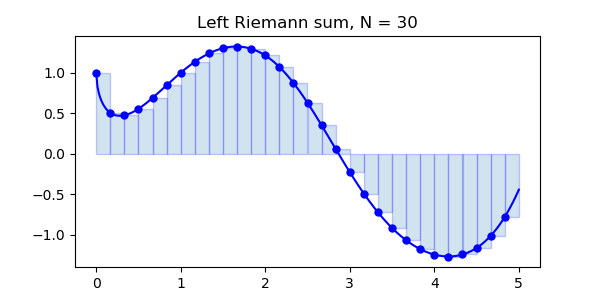
\includegraphics[width=\textwidth]{figure/riemann_left.png}
        \caption{Left Riemann sum}
    \end{subfigure}
    \begin{subfigure}[b]{0.45\textwidth}
        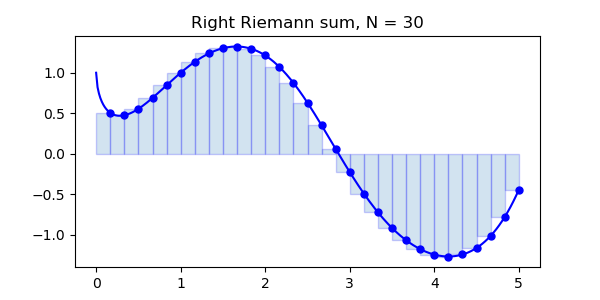
\includegraphics[width=\textwidth]{figure/riemann_right.png}
        \caption{Right Riemann sum}
    \end{subfigure}
    \begin{subfigure}[b]{0.45\textwidth}
        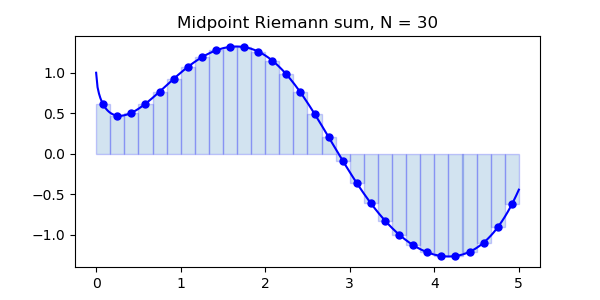
\includegraphics[width=\textwidth]{figure/riemann_mid.png}
        \caption{Midpoint Riemann sum}
    \end{subfigure}
    \begin{subfigure}[b]{0.45\textwidth}
        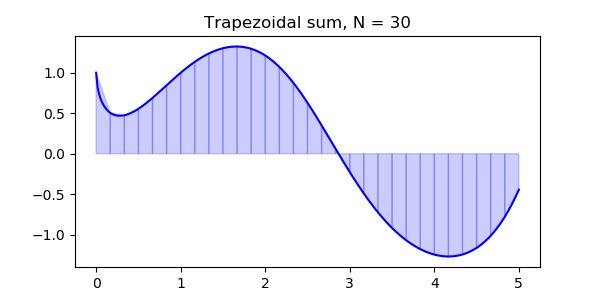
\includegraphics[width=\textwidth]{figure/riemann_trap.png}
        \caption{Trapezoidal sum}
    \end{subfigure}
    \caption{Riemann integration}
    \label{fig:Riemann_sum}
\end{figure}



\subsubsection{Newton-Cotes formulas}
\href{https://en.wikipedia.org/wiki/Newton-Cotes_formulas}{Newton–Cotes formulas}, also called the Newton–Cotes (quadrature) rules, are a group of formulas for numerical integration (also called quadrature) based on evaluating the integral at equally spaced points. If it is required that the points at which the integral is evaluated are not equally spaced, then other methods such as Gaussian quadrature are probably more suitable.

It is assumed that the value of a function $f$ defined on $[a;b]$ is known at equally spaced points $x_i$, for $i = 0, ..., n$, where $x_0 = a$ and $x_n = b$. There are two types of Newton–Cotes formulas, the ``closed'' type which uses the function value at all points, and the ``open'' type which does not use the function values at the endpoints. The Newton–Cotes formulas of degree $n$ are stated as:
\begin{align}
	\int_a^b f(x) dx &\approx \sum_{i=0}^{n} w_i f(x_i)   \quad \text{``close''} \\
	\int_a^b f(x) dx &\approx \sum_{i=1}^{n-1} w_i f(x_i) \quad \text{``open''}
\end{align}
where $x_i = ih + x_0$ with $h = \frac{x_n - x_0}{b} = \frac{b - a}{n}$ is called the step size. The $w_i$ are called weights and are derived from the Lagrange basis polynomials. They depend only on the $x_i$ and not on the function $f$. Let $L(x)$ be the interpolation polynomial in the Lagrange form for the given data points $(x_0, f(x_0)), ..., (x_n, f(x_n))$, then:
\begin{equation}
	\int_a^b f(x) dx \approx \int_a^b L(x) dx = \int_a^b \left( \sum_{i=0}^n f(x_i) l_i(x) \right) dx = \sum_{i=0}^n f(x_i) \underbrace{\int_a^b l_i(x) dx}_{w_i}
\end{equation}

The Newton-Cotes formulas, in fact, cover some other rules such as Riemann midpoint, trapezoidal sum, Simpson's rule... The following table lists some of the Newton-Cotes formulas (the notation $f_i$ is the shorthand for $f(x_i) = f(a + i \frac{b-a}{n}$):
\begin{table}[H]
\begin{center}
\caption{Numerical integration with Newton-Cotes formulas}
\begin{tabular}{cclll}
\multicolumn{5}{c}{Closed Newton-Cotes formulas}                                                                              \\
Degree $n$ & Step size $h$   & Common name       & Formula                                 & Error bound                      \\
\hline
1          & $b-a$           & Trapezoid rule    & $\frac{h}{2} (f_0 + f_1)$               & $\frac{1}{12} h^3 f^{(2)}(\xi)$  \\
2          & $\frac{b-a}{2}$ & Simpson's rule    & $\frac{h}{3} (f_0 + 4f_1 + f_2)$        & $\frac{1}{90} h^5 f^{(4)}(\xi)$  \\
3          & $\frac{b-a}{3}$ & Simpson's 38 rule & $\frac{3h}{8} (f_0 + 3f_1 + 3f_2 + f_3)$ & $\frac{3}{80} h^5 f^{(4)}(\xi)$  \\
           &                 &                   &                                         &                                  \\
\multicolumn{5}{c}{Open Newton-Cotes formulas}                                                                                \\
Degree $n$ & Step size $h$   & Common name       & Formula                                 & Error bound                      \\
\hline
2          & $\frac{b-a}{2}$ & Midpoint rule     & $2h f_1$                                & $\frac{1}{3} h^3 f^{(2)}(\xi)$   \\
3          & $\frac{b-a}{3}$ & Trapezoid rule    & $\frac{3h}{2} (f_1 + f_2)$              & $\frac{1}{4} h^3 f^{(2)}(\xi)$   \\
4          & $\frac{b-a}{4}$ & Milne's rule      & $\frac{4h}{3} (2f_1 - f_2 + 2f_3)$      & $\frac{28}{90} h^5 f^{(4)}(\xi)$
\end{tabular}
\end{center}
\end{table}



\subsubsection{Monte-Carlo integration}
Monte-Carlo integration uses random sampling of a function to numerically compute an estimate of its integral. Suppose that we want to integrate the one-dimensional function $f(x)$ from $a$ to $b$:
\begin{equation}
	F = \int_a^b f(x) dx
\end{equation}
We can approximate this integral by averaging samples of the function $f$ at uniform random points within the interval. Given a set of $N$ uniform random variables $X_i \in [a;b)$ with a corresponding PDF of $\frac{1}{b-a}$, the Monte Carlo estimator for computing $F$ is:
\begin{equation}
	\langle F^N \rangle = (b-a) \frac{1}{N-1} \sum_{i=0}^N f(X_i)
\end{equation}
The random variable $X_i \in [a;b)$ can be constructed by warping a random number uniformly distributed between zero and one, $\xi \in [0;1)$:
\begin{equation}
	X_i = a + \xi (b-a)
\end{equation}
Using this construction, we can expand the estimator to:
\begin{equation}
	\langle F^N \rangle = (b-a) \frac{1}{N} \sum_{i=0}^{N-1} f(a + \xi (b-a))
\end{equation}
Sine $\langle F^N \rangle$ is a function of $X_i$, it is also a random variable; and therefore, $\langle F^N \rangle$ is an approximation of $F$ using $N$ samples.

It is possible to show that:
\begin{equation}
	E \left[ \langle F^N \rangle \right] = F \quad \text{note that } pdf(F) = \frac{1}{b-a}
\end{equation}
As we increase the number of samples $N$, the estimator $\langle F^N \rangle$ becomes closer approximation of $F$. Due to the \textit{Law of Large Numbers}, in the limit we can guarantee that we have the exact solution:
\begin{equation}
	Pr \left\{ \lim_{N \rightarrow \infty} \langle F^N \rangle = F \right\} = 1
\end{equation}
We can estimate convergence of this estimation by determining the convergence rate of the estimators variance. It is possible to show that:
\begin{equation}
	\sigma \left[ \langle F^N \rangle \right] \propto \frac{1}{\sqrt{N}}
\end{equation}
This means that we must quadruple the number of samples in order to reduce the error by half. Standard integration techniques exist which converge much faster in one dimension, that's why Monte-Carlo integration is not a preference in one-dimensional problem. However the convergence rate of basic techniques becomes exponentially worse with increased dimensions; whereas the basic Monte Carlo estimator above can easily be extended to multiple dimensions, Algorithm \ref{algo:mc_inte}, and the convergence rate for Monte Carlo is independent of the number of dimensions in the integral. This makes Monte Carlo integration the only practical technique for many high dimensional integration problems. More details information on the Monte-Carlo integration can be found \href{https://cs.dartmouth.edu/~wjarosz/publications/dissertation/appendixA.pdf}{here} and \href{https://en.wikipedia.org/wiki/Monte_Carlo_integration}{here}.

\vspace{\baselineskip}
\begin{algorithm}[H]
\caption{Monte-Carlo integration}
\label{algo:mc_inte}  
\Begin{
    $x_{\min}, x_{\max}, y_{\min}, y_{\max}$  \tcc*[r]{Input} 
    Function $f(x,y)$, Number of sample $N$   \\
    Set temporary variable $tmp = 0$          \tcc*[r]{Initialisation}
    \For{$i = 1 \rightarrow N$}{
    	$x = \text{random.uniform} \in [x_{\min}; x_{\max}]$   \\
    	$y = \text{random.uniform} \in [y_{\min}; y_{\max}]$   \\
    	$tmp \mkern9mu +\!= f(x,y)$
	}
	$estimator = (x_{\max} - x_{\min}) (y_{\max} - y_{\min}) \frac{tmp}{N}$
} 
\end{algorithm}
\vspace{\baselineskip}

Another way of implementing the Monte-Carlo integration, following closely a counting-approach and geometrical definition of the integral can be found in Algorithm \ref{algo:mc_inte_1d}. This algorithm is, however, harder to generalize into multiple dimensions. 

\vspace{\baselineskip}
\begin{algorithm}[H]
\caption{Monte-Carlo integration by geometrical counting}
\label{algo:mc_inte_1d}  
\Begin{
    $x_{\min}, x_{\max}$                                        \tcc*[r]{Input} 
    Function $f(x)$, Number of sample $N$                       \\
    Finding bounds of $f(x) = f_{\min}, f_{\max}$               \tcc*[r]{Initialisation}
    Set counting variable $count = 0$, indicator vector $z$ (can be zero-initialized here) \\
    \For{$i = 1 \rightarrow N$}{
    	$x  = \text{random.uniform} \in [x_{\min}; x_{\max}]$   \\
    	$fx = f(x)$                                             \\
    	$ft = \text{random.uniform} \in [f_{\min}; f_{\max}]$   \\
    	\uIf{$|ft| \leq |fx|$}{
    		\If{$ft > 0$ \text{and} $fx > 0$ \text{and} $ft < fx$}{
    			$count \mkern9mu +\!= 1$               \tcc*[r]{area over x-axis is positive}
    			$\mathbf{z}[i] = 1$
    		}
    		\If{$ft < 0$ \text{and} $fx < 0$ \text{and} $ft \geq fx$}{
    			$count \mkern9mu -\!= 1$               \tcc*[r]{area under x-axis is negative}  
    			$\mathbf{z}[i] = -1$
    		}
    	}
    	\Else{
    		$\mathbf{z}[i] = 0$
    	}
	}
	$estimator = (x_{\max} - x_{\min}) (y_{\max} - y_{\min}) \frac{count}{N}$  \\
	Plotting with the indicator vector $\mathbf{z}$
} 
\end{algorithm}
\vspace{\baselineskip}

Figure \ref{fig:mc_inte_1d} presents the Monte-Carlo integration following Algorithm \ref{algo:mc_inte_1d} for an integral:
\begin{equation}
	\int_{10}^{20} x^2 \sin(x)^3 dx
\end{equation}
The results for a sample of 100.000 sample points following Algorithm \ref{algo:mc_inte} and \ref{algo:mc_inte_1d} are -181.04 and -182.12, respectively. The results from \href{https://www.wolframalpha.com/input/?i=integrate+x^2+sin^3+x+dx+from+10+to+20}{WolframAlpha} is -181.16. The approximation of this integral by the Riemann sum with 10.000 interval yields the result of -181.16. This example can be found \href{https://github.com/chitn/quantfin_study/blob/master/integration.py}{here}.

\begin{figure}[H]
    \centering
    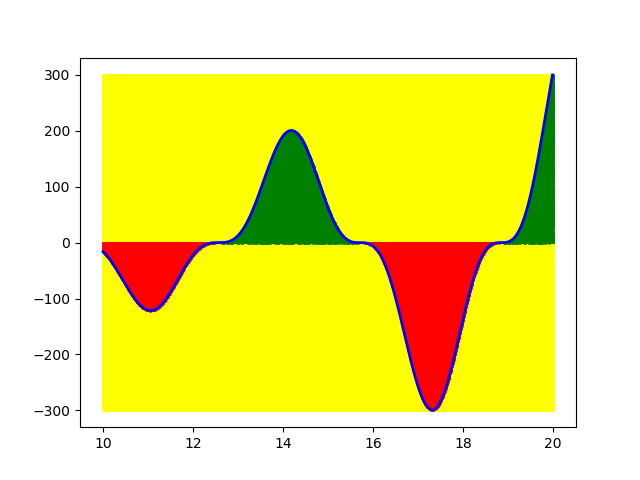
\includegraphics[width=0.75\textwidth]{figure/monte_carlo_inte.png}
    \caption{Monte-Carlo integration}
    \label{fig:mc_inte_1d}
\end{figure}



\subsection{Numerical differentiation}

\subsubsection{Derivative and differentiation}
The \href{https://en.wikipedia.org/wiki/Derivative}{derivative} of a function of a real variable measures the sensitivity to change of the function value (output value) with respect to a change in its argument (input value). Differentiation is the action of computing a derivative. The derivative of a function $y = f(x)$ of a variable $x$ is a measure of the rate at which the value $y$ of the function changes with respect to the change of the variable $x$. By definition we have:
\begin{equation}
	f'(a) = \lim_{h \rightarrow 0} \frac{f(a+h) - f(a)}{h}
\end{equation}
When the limit exists, $f$ is said to be differentiable at $a$. The derivative satisfies the property that:
\begin{equation}
	\lim_{h \rightarrow 0} \frac{f(a+h) - (f(a) + f'(a) \times h)}{h} = 0
\end{equation}
which means:
\begin{equation}
	f(a+h) \approx f(a) + f'(a) h
\end{equation}
for $f$ near $a$. This interpretation can be extended further easily. For example, if $f$ is twice differentiable then:
\begin{equation}
	f(a+h) \approx f(a) + f'(a) h + \frac{1}{2} f''(a) h^2
\end{equation}
If $f$ is infinitely differentiable, then this is the beginning of the Taylor series for $f$ evaluated at $a+h$ around $a$. Consequently, the simplest method to estimate the derivatives to an arbitrary order of accuracy is to use \href{https://en.wikipedia.org/wiki/Numerical_differentiation}{finite difference approximations} which can be central, forward or backward.



\subsubsection{First derivative}
Following the finite difference approximations, the first derivative is calculated as follows:
\begin{itemize}
	\setlength\itemsep{0em}
	\item The forward difference formula with step size $h$
	\begin{equation}
		f'(a) \approx \frac{f(a+h) - f(a)}{h}
	\end{equation}
	\item The backward difference formula
	\begin{equation}
		f'(a) \approx \frac{f(a) - f(a-h)}{h}
	\end{equation}
	\item The central difference formula is the average of the forward and backwards difference formulas
	\begin{equation}
		f'(a) \approx \frac{f(a+h) - f(a-h)}{2h}
	\end{equation}
\end{itemize}
It can be seen that the finite difference approximations are based on the Taylor series, therefore the error in the finite difference approximations can be derived from Taylor's theorem:
\begin{itemize}
	\setlength\itemsep{0em}
	\item The error of the forward difference formula
	\begin{equation}
		\left| \frac{f(a+h) - f(a)}{h} - f'(a) \right| \leq \frac{h F}{2}
	\end{equation}
	with $|f''(x)| \leq F$ for all $x in [a;a+h]$. This error formula is hold for the backward difference formula as well.
	\item The error of the central difference formula
	\begin{equation}
		\left| \frac{f(a+h) - f(a-h)}{2h} - f'(a) \right| \leq \frac{h^2 C}{6}
	\end{equation}
	with $|f'''(x)| \leq C$ for all $x in [a-h;a+h]$.
\end{itemize}
An important consideration in practice when the function is calculated using floating-point arithmetic is the choice of step size $h$. If $h$ is too small, the subtraction will yield a large rounding error due to cancellation. If $h$ is too large, apparently, the accuracy reduces. For the numerical derivative formula evaluated at $x$ and $x + h$, a choice for $h$ that is large enough to avoid the large rounding error of $\sqrt{\varepsilon}x$, where the machine epsilon $\varepsilon = 2.2 \times 10^{-16}$ but small enough to avoid the secant error for optimum accuracy; such an option can be:
\begin{equation}
	h = \sqrt{\varepsilon \left| \frac{f(x)}{f''(x)} \right|}
\end{equation}

In the family of the finite difference approximations, you can achieve approximation with higher order of accuracy by involving more terms of the Taylor series or \href{https://en.wikipedia.org/wiki/Finite_difference_coefficient}{finite difference coefficient}.



\subsubsection{Higher derivative}
Approximations of higher derivatives $f''(x), f'''(x),...$ can easily be obtained in by using the Talor series expansion as above. For example, the central difference formula for the second derivative is as follows:
\begin{align}
	f(a+h) &= f(a) + hf'(a) + h^2\frac{f''(a)}{2!} + h^3\frac{f'''(a)}{3!} + h^4\frac{f^{(4)}(\xi_+)}{4!} ... \nonumber \\
	f(a-h) &= f(a) - hf'(a) + h^2\frac{f''(a)}{2!} - h^3\frac{f'''(a)}{3!} + h^4\frac{f^{(4)}(\xi_-)}{4!} ... \nonumber \\
	\rightarrow f(a+h) + f(a-h) &= 2f(a) + h^2f''(a) + h^4 \frac{f^{(4)}(\xi_+) + f^{(4)}(\xi_-)}{24} \nonumber \\
	\rightarrow f''(a) &\approx \frac{f(a+h) - 2f(a) + f(a-h)}{h^2}
\end{align}
and the error term is:
\begin{equation}
	h^2 \frac{f^{(4)}(\xi_+) + f^{(4)}(\xi_-)}{24}
\end{equation}
in which $\xi_{+/-}$ is a small number between $a$ and $a+h$.

Other forms with the same or higher order of accuracy of finite difference formulas can be found \href{https://en.wikipedia.org/wiki/Finite_difference_coefficient}{here}.



\subsubsection{Partial derivatives}
Given a function of multiple variables, differentiation generalises in a simple way: differentiating the resulting function as a function of one variable while keeping other variable fixed. Finite difference formulas for partial derivatives follows the same approach. For example, the central difference formulas for a function of two variables are as follows:
\begin{align}
	\frac{\partial f}{\partial x}(a,b) &\approx \frac{f(a+h,b) - f(a-h,b)}{2h}  \\
	\frac{\partial f}{\partial y}(a,b) &\approx \frac{f(a,b+k) - f(a,b-k)}{2k}  \\
	\frac{\partial^2 f}{\partial x^2}(a,b) &\approx \frac{f(a+h,b) - 2f(a,b) + f(a-h,b)}{h^2}  \\
	\frac{\partial^2 f}{\partial x \partial y}(a,b) &\approx \frac{f(a+h,b+k) - f(a+h,b-k) - f(a-h,b+k) + f(a-h,b-k)}{4hk} 	
\end{align}    
Sometimes, the notation:
\begin{alignat*}{4}
	& f(a+h,b+k) &&= f_{1,1}  && \quad f(a+h,b-k) &&= f_{1,-1}  \\
	& f(a-h,b+k) &&= f_{-1,1} && \quad f(a-h,b-k) &&= f_{-1,-1} 
\end{alignat*}
is used in \href{https://www.uio.no/studier/emner/matnat/math/MAT-INF1100/h07/undervisningsmateriale/kap7.pdf}{practice}, then the finite difference formula for partial derivatives can be shortened, for example:
\begin{equation}
	\frac{\partial^3 f}{\partial x^2 \partial y} \approx \frac{f_{2,1} - 2f_{0,1} + f_{-2,1} - f_{2,-1} + f_{0,-1} - f_{-2,-1}}{8h^2k}
\end{equation}

\begin{center}
\begin{footnotesize}
\fbox{
\begin{minipage}{0.90\textwidth}

\href{http://www.ohiouniversityfaculty.com/youngt/IntNumMeth/lecture27.pdf}{\textbf{Example}}

Suppose $u = u(x,y)$ is a function of two variables that we only know at grid points $(x_i, y_j)$. The values of $u$ at $(x_i, y_j)$ are recorded in the matrix:
\begin{equation*}
	u(x_i, y_j) = 
	\begin{pmatrix}
		5.1 & 6.5 & 7.5 & 8.1 & 8.4  \\
		5.5 & 6.8 & 7.8 & 8.3 & 8.9  \\
		5.5 & 6.9 & 9.0 & 8.4 & 9.1  \\
		5.4 & 9.6 & 9.1 & 8.6 & 9.4
	\end{pmatrix}
\end{equation*}
Suppose that the grid points are evenly spaced in both $x-$ and $y-$direction with $h = 0.5$ and $k = 0.2$. Then $u_y(x_2, y_4)$ can be approximated by the central difference as follows:
\begin{equation*}
	u_y(x_2, y_4) \approx \frac{u_{2,5} - u_{2,3}}{2k} \approx \frac{8.9 - 7.8}{2 \times 0.2} = 2.75
\end{equation*}

Similarly, $u_{xy}(x_2, y_4)$ can be approximated as:
\begin{equation*}
	u_{xy}(x_2, y_4) \approx \frac{u_{3,5} - u_{3,3} - u_{1,5} + u_{1,3}}{4hk} \approx \frac{9.1 - 9.0 -8.4 + 7.5}{4 \times 0.2 \times 0.5} = -2.0
\end{equation*}

\end{minipage}
}
\end{footnotesize}
\end{center}

Figure \ref{fig:nume_deriv} presents the first and second derivative of a function calculated by the numerical differentiation with the finite difference approach. The implementation can be found \href{https://github.com/chitn/quantfin_study/blob/master/differentiation.py}{here}.

\begin{figure}[H]
    \centering
    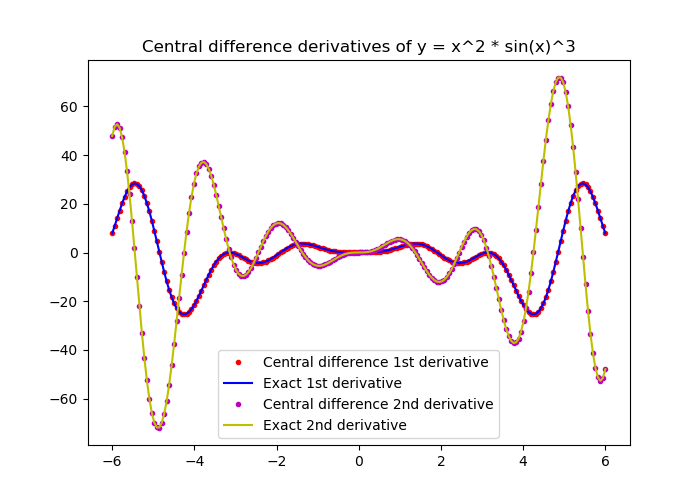
\includegraphics[width=0.75\textwidth]{figure/derivative.png}
    \caption{First and second derivatives calculated with numerical differentiation}
    \label{fig:nume_deriv}
\end{figure}



\subsection{Root finding}
In mathematics and computing, a \href{https://en.wikipedia.org/wiki/Root-finding_algorithms}{root-finding algorithm} is an algorithm for finding zeroes of continuous functions, i.e. a number/vector $x$ for which $f(x) = 0$. Generally, the zeroes of a function cannot be computed exactly nor expressed in closed form, root-finding algorithms provide approximations to those. There are many algorithms for finding roots, this section only describes three basic algorithms, namely:
\begin{itemize}
	\setlength\itemsep{0em}
	\item Bisection method
	\item Newton-Raphson method
	\item Secant method
\end{itemize}
The implementation of these algorithms can be found \href{https://github.com/chitn/quantfin_study/blob/master/root_finding.py}{here}.



\subsubsection{Bisection method}
The simplest root-finding algorithm is the \href{https://en.wikipedia.org/wiki/Bisection_method}{bisection method} which can apply to any continuous function $f(x)$ on an interval $[a;b]$ where the value of the function $fx)$ changes sign from $a$ to $b$, i.e. $f(a) \times f(b) < 0$. The idea is simple: divide the interval in two, a solution must exist within one sub-interval, select the sub-interval where the sign of $f(x)$ changes and repeat until the root is found. Following this algorithm, we can easily estimate the absolute error of the approximation after $N$ iteration as:
\begin{equation}
	\left| x_{\text{exact}} - x_N \right| \leq \frac{b - a}{2^{N+1}}
\end{equation}
From this equation, we can also calculate the minimum number of iteration required to achieve the absolute error less than a certain threshold $\epsilon$ as follows:
\begin{equation}
	N \geq \frac{\log{\frac{b-a}{\epsilon}}}{\log(2)} - 1
\end{equation}
Although Bisection method is easy to implement and quite robust, generalization of Bisection method to a multivariate problem is not straightforward. 



\subsubsection{Newton-Raphson method}
\href{https://en.wikipedia.org/wiki/Newton's_method}{Newton–Raphson method} is a root-finding algorithm which produces successively better approximations to the roots of a real-valued function.  
\\


\textbf{Single-variable function}

Given a single-variable function $f(x)$, the function's derivative $f'(x)$ and an initial guess $x_0$ for a root of $f(x) = 0$. If the initial guess is close enough, then:
\begin{equation}
	x_1 = x_0 - \frac{f(x_0)}{f'(x_0)}
\end{equation}
is a better approximation of the root than $x_0$. Geometrically, $(x_1,0)$ is the intersection of the $x$-axis and the tangent of the graph $f$ at a point $(x_0,f(x_0))$, therefore, the improved guess is the root of the linear approximation at the initial point. The process is repeated as:
\begin{equation}
	x_{n+1} = x_n - \frac{f(x_n)}{f'(x_n)}
\end{equation}
until $\left| x_{n+1} - x_n \right| \leq \epsilon$ in which $\epsilon$ is a certain predefined precision. Newton-Raphson method will usually converge with a quadratic rate provided that the initial guess is close enough to the unknown root and that $f'(x_0) \neq 0$.
\\

 
\textbf{Multivariate problem}

Given $k$ multivariate functions $\mathbf{f} = (f_1, f_2,... f_k)$ of $k$ variables $\mathbf{x} = (x_1, x_2,... x_k$. One can find the root $\mathbf{x}$ satisfying $\mathbf{f(x)} = 0$ by following the iteration:
\begin{equation}
	\mathbf{x}_{n+1} = \mathbf{x}_{n} - \mathbf{J}_{\mathbf{f}} (\mathbf{x}_n)^{-1} \mathbf{f}_{\mathbf{x}_n}
\end{equation}
in which $\mathbf{J}_{\mathbf{f}}$ is the Jacobian matrix which is defined as:
\begin{equation}
	\mathbf{J}_{\mathbf{f}} = \left[ \frac{\partial \mathbf{f}}{\partial x_1} \dots \frac{\partial \mathbf{f}}{\partial x_n} \right] =
	\begin{bmatrix}
		\frac{\partial f_1}{\partial x_1} & \dots & \frac{\partial f_1}{\partial x_n} \\
		\vdots & \ddots & \vdots \\
		\frac{\partial f_n}{\partial x_1} & \dots & \frac{\partial f_n}{\partial x_n}		
	\end{bmatrix}
\end{equation}
Rather than computing the inverse of the Jacobian matrix, we can save time by solving the system of linear equations:
\begin{equation}
	\mathbf{J}_{\mathbf{f}} (\mathbf{x}_n) \left( \mathbf{x}_{n+1} - \mathbf{x}_n \right) = -\mathbf{f} (\mathbf{x}_n)
\end{equation}
for the unknown $\mathbf{x}_{n+1} - \mathbf{x}_n$.
\\


\textbf{Minimization and maximization problems}

Newton-Raphson method can be used to find a minimum or maximum of a function $f(x)$. The derivative is zero at a minimum or maximum, so local minima and maxima can be found by applying Newton-Raphson method to the derivative. The iteration becomes:
\begin{equation}
	x_{n+1} = x_n - \frac{f'(x_n)}{f''(x_n)}
\end{equation}
\\


\textbf{Practical considerations}

Newton-Raphson method is an extremely powerful technique, in general the convergence is quadratic. However, there are a couple of difficulties with the method:
\begin{itemize}
	\setlength\itemsep{0em}
	\item Difficulty in calculating derivative of a function: we can use numerical approximation of the derivative or use secant method;
	\item Failure to converge to the root;
	\item Overshoot then divergence;
	\item Poor initial estimation then divergence;
	\item and some other minor problems. 
\end{itemize}
This mean we need pay enough attention on using Newton-Raphson method. More information on the problems with Newton-Raphson method and how to (partially) overcome them can be found \href{https://en.wikipedia.org/wiki/Newton's_method}{here}.



\subsubsection{Secant method}
The \href{https://en.wikipedia.org/wiki/Secant_method}{secant method} is very similar to the bisection method except instead of dividing each interval by choosing the midpoint the secant method divides each interval by the secant line connecting the endpoints. The secant method can be thought of as a finite-difference approximation of Newton-Raphson method although it is invented long before. The secant method always converges to a root of $f(x) = 0$ provided that $f(x)$ is continuous on $[a;b]$ and $f(a) \times f(b) < 0$.

The secant method can be birefed as follows: given a function $f(x)$ and the interval $[a_0; b_0]$, compute $f(x_0)$ where $x_0$ is given by the secant line:
\begin{equation}
	x_0 = a_0 - f(a_0) \frac{b_0 - a_0}{f(b_0) - f(a_0)}
\end{equation}
Then determine the next subinterval which should be $[a_0; x_0]$ if $f(a_0) \times f(x_0) < 0$ or $[x_0; b_0]$ if $f(x_0) \times f(b_0) < 0$. Repeat this procedure until the root is found. 
\\

Table \ref{tab:root_finding} presents the performance of the aforementioned root-finding algorithms in finding the root of function:
\begin{equation}
	f(x) = \sqrt{x} * \log(x) - 5
	\nonumber
\end{equation}
in the interval of $[1;10]$ with the threshold for the absolute error of $\epsilon = 10^{-10}$. The implementation of this illustration can be found \href{https://github.com/chitn/quantfin_study/blob/master/root_finding.py}{here}.
\begin{table}[H]
\begin{center}
\caption{Performance of root-finding algorithms}
\label{tab:root_finding}
\begin{tabular}{lccc}
Method                    & Iteration number & Root      & Error                    \\
\hline
Bisection method          & 33               & 6.8017009 & 3.9394 $\times 10^{-11}$ \\
Newton-Raphson numerical  & 4                & 6.8017009 & 4.3432 $\times 10^{-13}$ \\
Newton-Raphson analytical & 4                & 6.8017009 & 8.8818 $\times 10^{-16}$ \\
Secant method             & 11               & 6.8017009 & 4.4653 $\times 10^{-11}$
\end{tabular}
\end{center}
\end{table}

















